\documentclass{article}
\usepackage{ctex}
\usepackage{tikz}
\usepackage{amsmath}

\title{大物作业}
\author{张博涵-应化1903(学号:1912020312)}
\date{\today}

\begin{document}

	\maketitle
	
	由题意可知,小珠离开环的底部停止\\在环上的某一点,此时它应该如右图受力方式:
	%
	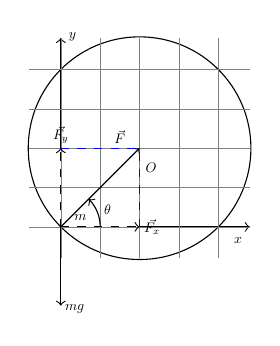
\begin{tikzpicture}
		\draw[->] (0,-1) --node[scale=0.5][near end,right=0.4cm,below = 0.15cm]{$x$} (1.4,-1);
		\draw[->] (-1,0) --node[scale=0.5][near end,right =0.3cm,above = 0.5cm]{$y$} (-1,1.4);
		\draw (0,0) circle (1.414cm);
		\draw[step=.5cm,gray,very thin] (-1.4,-1.4) grid (1.4,1.4);
		\draw[->] (-1,-1) --node[scale=0.5][near start,below=2pt]{$m$}node[scale=0.5][near end,right=15pt]{$O$}
		    node[scale=0.5][near end,above=14pt]{$\vec{F}$} (0,0);
		\draw[->] (-1,-1) --node[scale=0.5][near end,right=10pt,below=10pt]{$mg$}  (-1,-2);
		\draw[dashed][->](-1,-1) --node[scale=0.5][near end,above=14pt]{$\vec{F_y}$} (-1,0);
		\draw[dashed][->](-1,-1) --node[scale=0.5][near end,right=14pt]{$\vec{F_x}$} (0,-1);
		\draw[dashed , blue](-1,0) -- (0,0);
		\draw[dashed , blue](0,-1) -- (0,0);
		\draw[->](-0.5,-1) arc  (0:45:0.5);
		\draw node[scale=0.5][below = 1.55cm,left = 0.6cm]{$\theta$};
		 
	\end{tikzpicture}\\
	%
	
	
	对圆环给小珠的弹力$\vec{F}$进行分解,设$\vec{F}$的大小为$F$,分解为一个水平方向的力$\vec{F_x}$和一个竖直方向的力$\vec{F_y}$
	
	其中\quad$\vec{F_x}=F_x \vec{i}$\quad,\quad $\vec{F_y}=F_y \vec{j}$
	\begin{equation}
		F_x=F\cos \theta\label{1}
	\end{equation}
	\begin{equation}
		F_y=F\sin \theta\label{2}
	\end{equation}
	竖直方向受力平衡,可得
	\begin{equation}
		F_y=mg\label{3}
	\end{equation}
	
	此时小珠随圆环绕竖直直线转动,作一个绕轴转动的匀速圆周运动,这个运动圆周的圆心在此小珠(视为质点)向竖直方向的投影点,圆周运动的半径设之为$R_1$,由数学知识可知:
	\begin{equation}
		R_1=R\cos \theta\label{4}
	\end{equation}
	此时可知,$\vec{F}$的分力$\vec{F_x}$用于提供该小珠随圆环绕竖直直线转动的向心力,则有:
	\begin{equation}
		F_x=m\omega^2R_1\label{5}
	\end{equation}
	连理上面的式子(\ref{1})$\sim$(\ref{5})可解得关系式(角速度$\omega$视之为正):
	$$\omega=\sqrt{\frac{g}{R \sin \theta}}$$
	由于三角函数$\sin \theta $是有界的,所以:
	$$\omega=\sqrt{\frac{g}{R \sin \theta}}\geq\sqrt{\frac{g}{R\times 1}}=\sqrt{\frac{g}{R}}$$
	
	\begin{flalign}
	 \mbox{答:}\quad \omega\mbox{最小应为}\sqrt{\frac{g}{R}} & & \nonumber 
	\end{flalign}
	
	
\end{document}